\documentclass{article}
\usepackage{pythonhighlight}
\usepackage{graphicx}
\usepackage{ctex}
\usepackage[left=3cm,top=3cm,right=3cm]{geometry}
\usepackage{hyperref}
% TITLE PAGE CONTENT %%%%%%%%%%%%%%%%%%%%%%%%
%%%%%%%%%%%%%%%%%%%%%%%%%%%%%%%%%%%%%%%%%%%%%
\newcommand{\labno}{06}
\newcommand{\labtitle}{EE208 Web.py}
\newcommand{\authorname}{周李韬}
\newcommand{\studentno}{518030910407}
\newcommand{\classno}{F1803016}
% END TITLE PAGE CONTENT %%%%%%%%%%%%%%%%%%%%


\begin{document}

\begin{center}
{\LARGE \textsc{Laboratory No. \labno:} \\ \vspace{4pt}}
{\Large \textsc{\labtitle} \\ \vspace{4pt}} 
\rule[13pt]{\textwidth}{1pt} \\ \vspace{15pt}
{\large By: \authorname \\ \vspace{10pt}
No. \studentno \\ \vspace{10pt}
SJTU \classno \\ \vspace{10pt}
\today \vspace{20pt}}
\end{center}



\section{实验准备}

\subsection{实验环境}
\begin{itemize}
\item\textbf{Environment} Ubuntu 16.04 (on Virtual Machine)
\item\textbf{Language} Python 2.7.16 with packages as follows
	\begin{itemize}
	\item urllib 1.24.2
	\item beautifulsoup4 4.8.0
	\item lucene 4.9.0
	\item web.py 3.7
	\end{itemize}
\item\textbf{Tools} PyCharm 2019.2, Virtual Box
\end{itemize}

\subsection{实验目的}
本实验中,我们需要为此前构建的索引和检索程序建立一个web前端。要求能够输入关键词、通过网页形式返回检索结果,本实验的实现基于Python中web.py库的框架。

\subsection{实验原理}

基于web.py库,要搭建搜索引擎前端,我们还需要设计URL的组织方式、生成页面的模板、并设计函数将用户的请求对接我们的检索程序并返回相应的检索结果。我们的前端包含两类页面,首页“index”和搜索结果页“s”。在index页面我们需要设计一个输入关键词的表单,这可以通过web.py中form类实现,用户输入信息keyword,按下Button后,表单会提交一个GET搜索结果页面的请求,web.py会根据参数keyword生成搜索结果“s”类的一个实例。具体而言,web前端会调用此前实验中搭建完成的检索程序,根据keyword从已建立的索引中查找匹配的文档,传入搜索结果页的模板中,生成用户需要的结果网页。以上两类页面的搭建构成了本次实验目标构建的一个简单搜索引擎。

需要注意的是,我们在此前的实验中,并没有在索引中存储HTML网页的文字内容“contents”,也没有设计检索程序返回contents的匹配摘要和关键词高亮展示。因此,在搭建网页之前,我们还需要重新建立带contents的索引,设计能够返回高亮关键词的文档摘要函数。

\section{实验步骤}

\subsection{搜索结果的高亮和摘要}

\subsubsection{Solution}

\paragraph{重建索引}

本实验的搜索结果网页要求返回网页内容中关键词的上下文,为此我们需要首先重建索引,将网页中的文本内容存储下来。我们修改Lab5中UpdateFiles.py脚本中FieldType配置,配置如下表所示。contents的FieldType被设置成与title一样被索引、存储、分词和记录词频位置。与此前的实验相同,我们采用了结巴中文分词器和Lucene库中的SimpleAnalyzer进行分词索引。

\begin{table}[h]
\begin{center}
\begin{tabular}{cccccc}
\hline
\textbf{Field Type} & \textbf{Field Name} & \textbf{Indexed} & \textbf{Stored} & \textbf{Tokenized} & \textbf{\begin{tabular}[c]{@{}c@{}}Record Freq\\ \& Position\end{tabular}} \\ \hline
\textbf{t1}         & path, url, name     & N                & Y               & N                  & N                                \\
\textbf{t2}         & \textbf{contents}, titles    & Y                & Y               & Y                  & Y                                \\
 \hline
\end{tabular}
\end{center}
\end{table}

这一部分中除了FieldType的配置,其他的代码都与Lab5中相同,因此不在此详述。


\paragraph{提取摘要和关键词}

我们提取内容摘要的基本原理如流程图\ref{fig:flowchart}所示,首先针对存储contents的文档,我们调用原有配置的analyzer获取contents的tokenStream。对文档的tokenStream,我们首先选用SimpleSpanFragmenter将文档内容分割成长度约为100字左右的若干片段,随后我们利用原本配置过的scorer进行打分,选取匹配query程度最高的片段,利用SimpleHTMLFormatter对其中的关键字进行标红的高亮处理,输出经过处理后的当前fragmenter。考虑到我们最终的实现是在网页中的,因此高亮处理的过程中,我们可以直接为关键词加上对应的HTML标签,达到高亮的效果。

\begin{figure}[htbp]
\centering
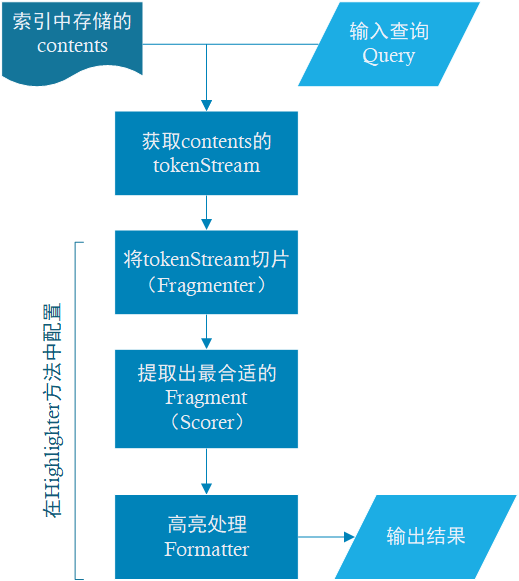
\includegraphics[width=10.5cm]{img/flowchart.png}
\caption{提取摘要和关键词的原理}
\label{fig:flowchart}
\end{figure}


配置Lucene中Highlighter实例的代码如下:
\begin{python}
scorer = QueryScorer(query)                                   # 对片段打分
fragmenter = SimpleSpanFragmenter(scorer)                     # 分割片段
simpleHTMLFormatter = SimpleHTMLFormatter("<b><font color='red'>", "</font></b>")
                                                              # 高亮处理
highlighter = Highlighter(simpleHTMLFormatter, scorer)        # 配置Highlighter
highlighter.setTextFragmenter(fragmenter)
\end{python}

对检索条目调用Highlighter方法的代码如下:
\begin{python}
results = []
for i, scoreDoc in enumerate(scoreDocs):
    doc = searcher.doc(scoreDoc.doc)
    contents = doc.get("contents");
    if contents :
        tkStream = analyzer.tokenStream("contents",contents)
        highlight = highlighter.getBestFragment(tkStream, contents)
    results.append((doc.get("title").strip(),doc.get("url"),highlight))
return results
\end{python}

\subsubsection{Results}
在本实验中经过重新搭建的搜索程序能够实现搜索文档内容摘要的输出和关键词的高亮。函数的输出结果是一个(标题,带高亮摘要,url)的tuple列表。在如图\ref{fig:highlightsearch}中,展示了一张测试截图。

\begin{figure}[htbp]
\centering
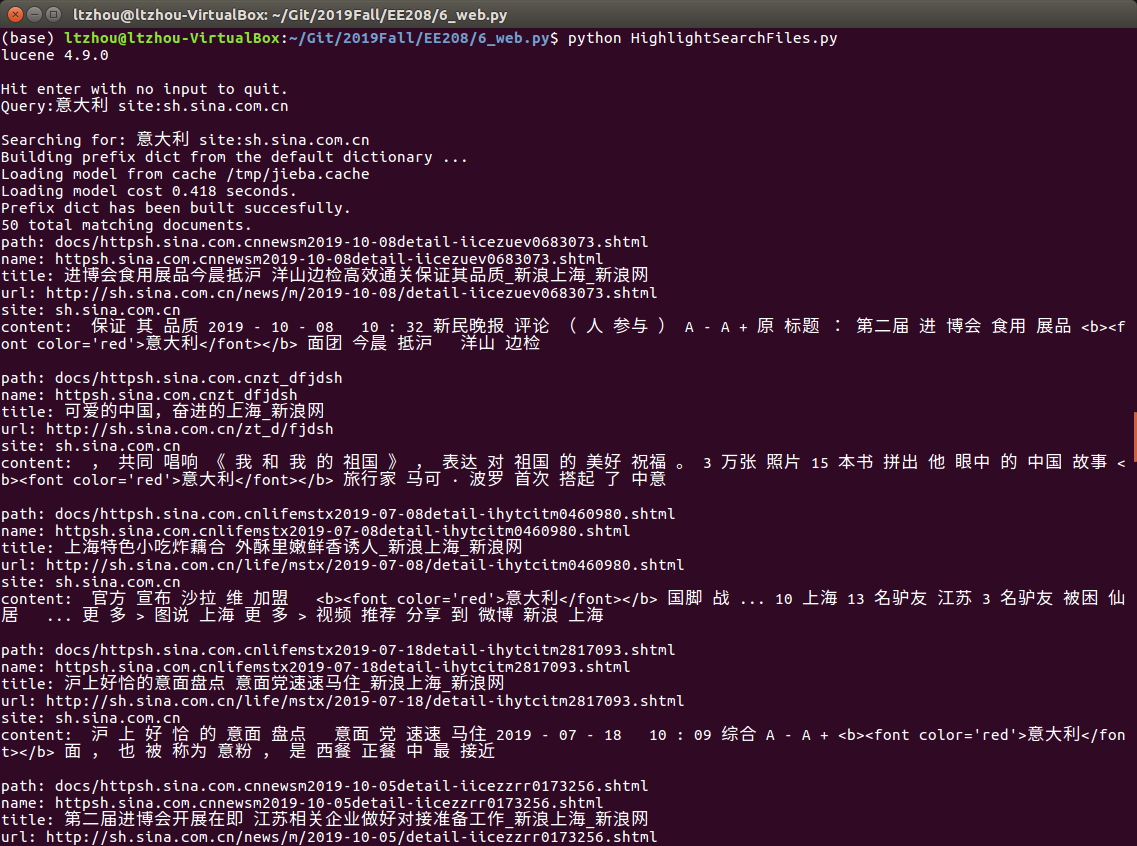
\includegraphics[width=14.5cm]{img/highlightsearch.png}
\caption{检索函数运行示例}
\label{fig:highlightsearch}
\end{figure}

\subsection{web的搭建}

\subsubsection{Solution}

\paragraph{URL的组织关系}
如原理中所示,实验中我们需要两类网页,搜索主页和结果页,分别匹配“\\”和'“\\s”两类URL。在web.py中的配置如下。
\begin{python}
urls = (
    '/', 'index',
    '/s', 's'
)
\end{python}

在两类页面中,我们都通过web.py中的Form类,在网页上提供了一个搜索框,用于接收用户输入的keyword,并跳转到相应地址。在web.py中,搜索框表单的配置如下。
\begin{python}
login = form.Form(
    form.Textbox('keyword'),
    form.Button('Search'),
)
\end{python}

模板中,为了使搜索框点击后跳转到搜索结果页面,我们在form标签中,加上了对应的GET请求参数。
\begin{python}
$def with(form)
<h1>Search</h1>
<form action="/s" method="GET">
    $:form.render()
</form>
\end{python}

在index模板中,模板的第一个参数就是我们创建的表单实例。
\begin{python}
class index:
    def GET(self):
        f = login()
        return render.formtest(f)
\end{python}

在搜索结果页中用类似的方法构造搜索框表单,我们就能实现主页与搜索结果页面间的组织。

\paragraph{搜索结果的输出}
用户只有通过提交搜索表单才会访问到搜索结果页,因此搜索结果页的URL中,一定会含有keyword的参数值。我们首先获取该参数。
\begin{python}
class s:
    def GET(self):
        user_data = web.input()
        vm_env.attachCurrentThread()
        f = login()
        kw = user_data.keyword
\end{python}

对该参数调用上一节中的检索函数,我们可以获得一串包含标题、高亮摘要、URL的搜索结果列表。我们设计了一个函数将这些内容通过HTML的标签组织起来。
\begin{python}
def func(command):
    result_seg = running(command)
    output = ''
    count = 0
    for item in result_seg:
        count += 1
        output += "<div id='res"+str(count)+"'>"
        output += "<h3><a href='"+item[1]+"'>"+item[0]+"</a></h3>"
        output += "<p>"+item[2]+"</p>"
        output += item[1]
        output += "</div>"
        output += "<hr>"
    return output
\end{python}

每一条搜索结果都由一个id为res[n]的分区组成,id的设置将方便于日后翻页功能的实现。div分区之间用一根分割线隔开,div内依次输出标题、带高亮的摘要和URL,其中,标题被a标签加上了指向网页实际地址的URL。将将该函数返回的内容传入模板页中,我们就实现了一个简单搜索结果页的搭建。

\begin{python}
contents = func(kw)
return render.result(f,kw,contents)
# result页面的三个参数分别是搜索框表单、关键词和搜索结果内容
\end{python}

\subsubsection{Result}

本实验中搭建的搜索前端在浏览器中的实例如图\ref{fig:exp1}和图\ref{fig:exp2}所示。

\begin{figure}[htbp]
\centering
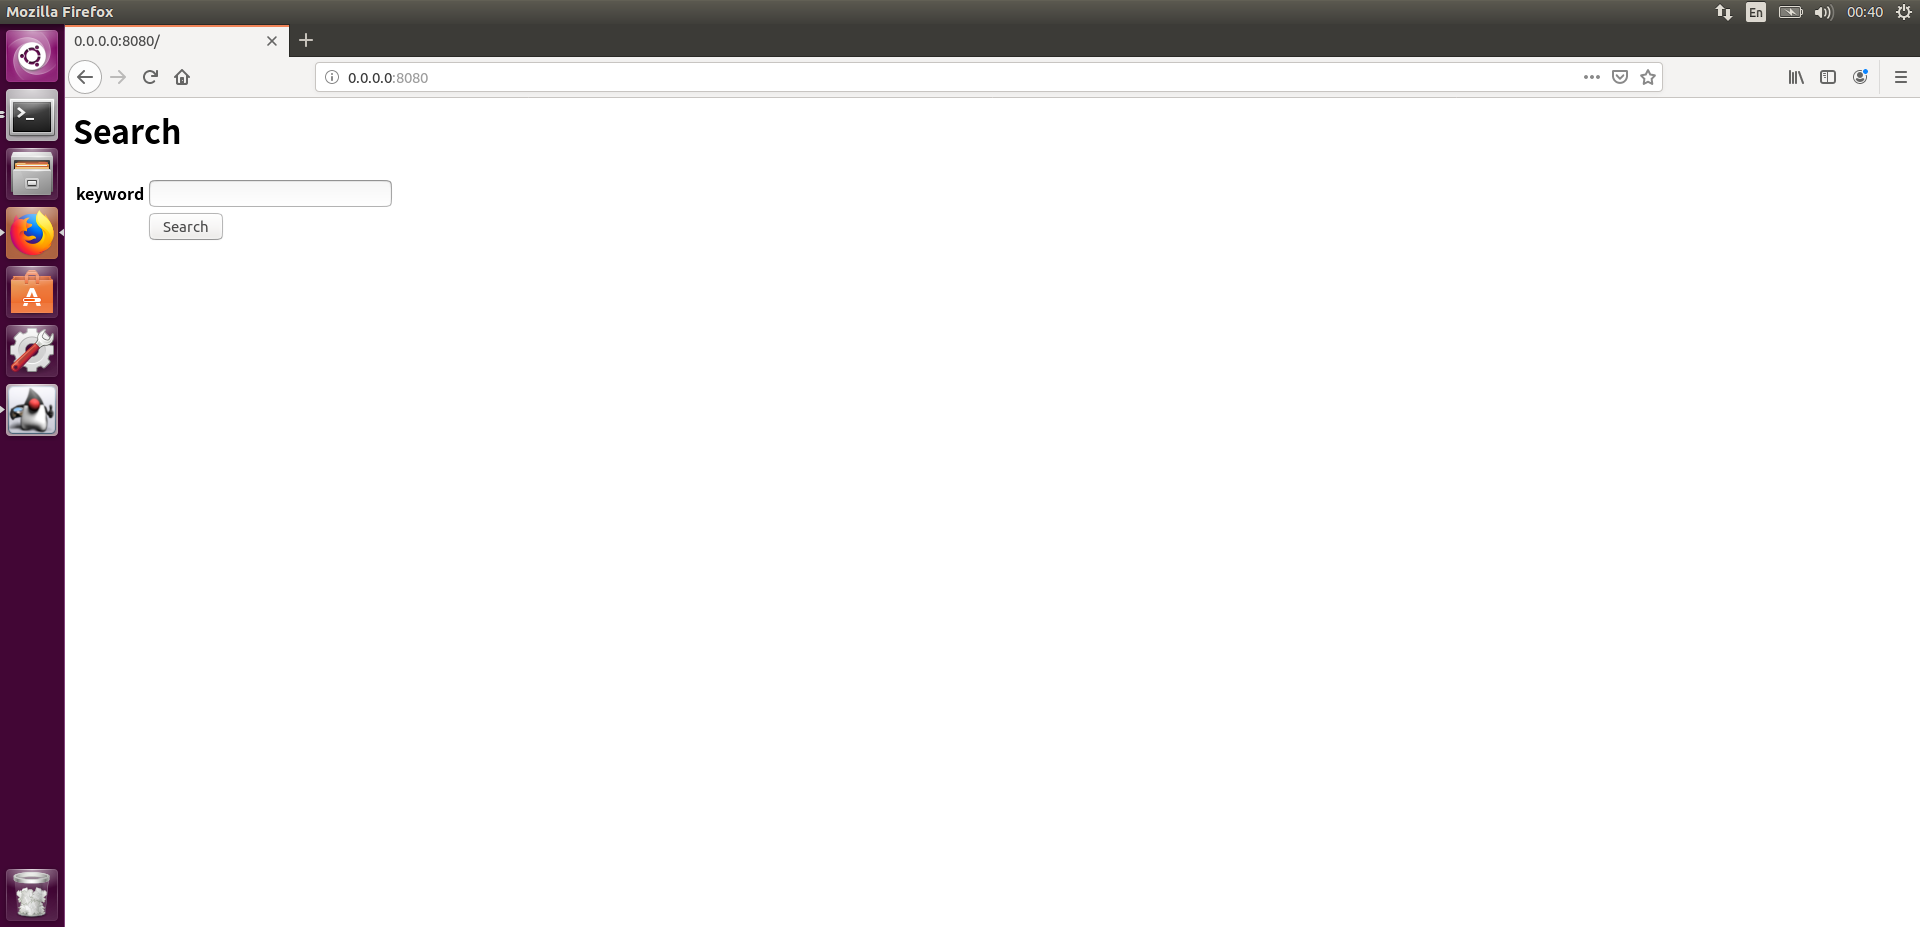
\includegraphics[width=14.5cm]{img/home.png}
\caption{前端主页}
\label{fig:exp1}
\end{figure}

\begin{figure}[htbp]
\centering
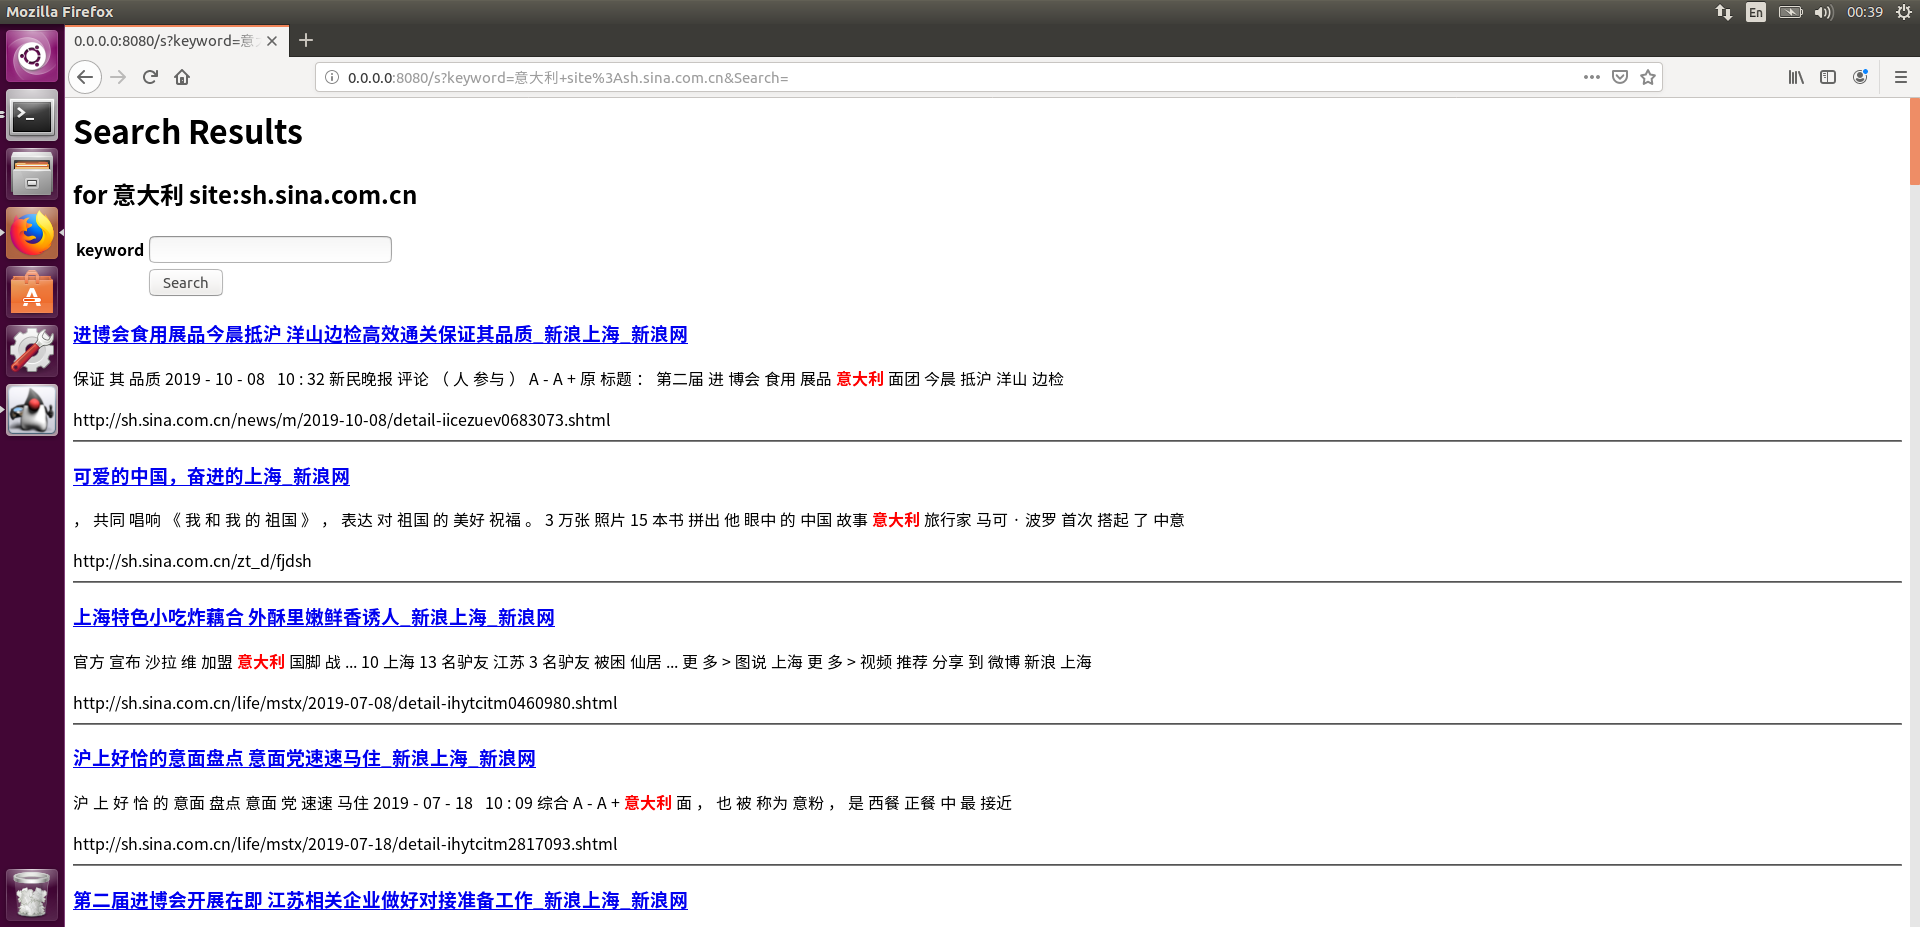
\includegraphics[width=14.5cm]{img/searchpage.png}
\caption{前端搜索结果页示例}
\label{fig:exp2}
\end{figure}


\section{实验总结}
\paragraph{概述}
本实验中,我们对Lab5中构造的支持site搜索的简单搜索引擎进行了前端的搭建,在搭建的过程中,我们重建了存储内容的索引,并且给出了能够返回带关键词高亮的摘要检索函数。

\paragraph{感想}
通过本次实验的学习,我更加熟练地掌握了搭建搜索引擎的技巧,并且通过web.py搭建网站的实践,对URL组织、GET/POST请求等概念有了更直观的认识。

\paragraph{创新}
在本实验中,除了搭建满足实验要求的网站外,我还为文本摘要加上了高亮显示。对网站的进一步美化和内容丰富将会在下一次中期整合Lab中叙述。

\paragraph{问题}
在利用template生成网页的过程实验过程中,虽然通过参数向web.py传入了一段HTML标签文本,但浏览器中没有对其进行解析,而是直接将代码输出。出现这一问题的原因在于,web.py中对传入参数有两种方法,通过\$传入的内容会直接以纯文本的方式输出在网页上,而只有通过\$:传入的内容才会被进行HTML解析。通过修改template中HTML模板的代码,该问题得以改正。

此外,最初在web.py中调用Lucene进行搜索时也会得到报错信息。这是因为Lucene使用的java虚拟机被错误地初始化或调用了。通过改写助教提供的示例代码后,该问题得到了解决。



\end{document}

